\section{Velocity Controller}\label{sec:velocity_controller}
The velocity controller node uses a linear function that is inversely proportional, which means that the function's product will be unchanged, to the distance from the customer who is using it. This means that the further the customer is away from the robot, the slower the robot will move to let the customer catch up to it. Equation \ref{eq:velocityFunction} shows the line function of the controller.

\begin{equation}
    Velocity = -(0.38 * distance\_from\_person) + 1.16
    \label{eq:velocityFunction}
\end{equation}

The line function were found by using two points that define the behaviour of the velocity controller. Point A(1.2, 0.7) where 1.2 defines the minimum distance to keep from the person and 0.7 defines the maximum velocity of the robot. Point B(3.0, 0) is the maximum distance between the robot and the person, and 0 is the velocity of the robot at that distance. Figure \ref{fig:velocity_controller_graph} shows a graph of the line equation.

\begin{figure}[H]
    \centering
    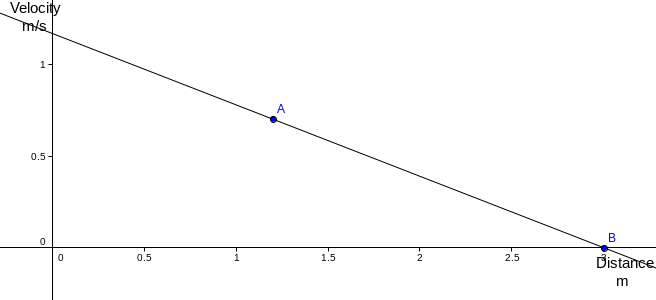
\includegraphics[width=0.9\textwidth]{figures/velocity_distance_graph.png}
    \caption{Graph showing the relation between the velocity of the robot and the distance from the person.}
    \label{fig:velocity_controller_graph}
\end{figure}

The node works by first subscribing to "sensorPosition" topic which is the output of the Kalman filter. The output is a point in the map indicating where the tracked person is in xy-plane. This point is then used to calculate the distance to the person from the "base\_link" frame of the robot. The velocity is then calculated and sent to the parameter server using the "dynamic\_reconfigure" package. If the distance to the customer is greater than 3 meters, the robot sends a request to the "move\_base" action server to cancel the current goal and the robot stops in place.